\section{Retained Original Numerical Experiments}
\label{app:legacy-experiments}
\begingroup
\color{blue}
\setlength{\emergencystretch}{2em}

{\color{blue}This appendix retains every original experimental figure and
table from the supplied manuscript, apart from the two-point energy example,
which remains in the main text as Table~\ref{tab:toy}. The results below are
historical comparisons, not additional fresh-draw repetitions of the new
experiments. They complement Appendix~\ref{app:additional-experiments} and
are kept to preserve the original evidence, including comparisons favorable
to competing methods.}


\subsection{Methods and Metrics}

We provide a comprehensive empirical validation of the proposed \emph{TSCP} method (Algorithm~\ref{alg:shortcut}) using simulated and real data. 
The performance of TSCP is compared to that of three representative benchmark approaches: (i) \emph{Unscaled Max}, a direct extension of split conformal inference that applies the $\ell_\infty$ norm to the residuals, summarized in Algorithm~\ref{alg:unscaled}; (ii) \emph{Point CHR}, a data-splitting variant recently proposed by \citet{sampson2024conformal}, which estimates per-target out-of-sample points using a held-out calibration set and adjusts them to form axis-aligned rectangular sets; (iii) \emph{Emp.~Copula}, the first distribution-free copula-based method introduced in \citet{messoudi2021copula}. 

The results of additional experiments comparing TSCP to different approaches are in Appendix~\ref{app:additional-experiments}.
We do not include in this empirical study alternative copula-based methods---e.g., vine copulas \citep{pmlr-v258-park25c}---because their main limitations relative to our approach are the same as those of the \emph{Emp.~Copula} benchmark.
To enable meaningful direct comparisons, we also omit approaches that do not produce rectangular prediction sets.

For simplicity, we apply all methods using the same conditional mean-regression model $\hat{f}$ and standard absolute residuals; i.e., $E_j(\mathbf X,Y_j)=|Y_j-\hat{f}_j(\mathbf X)|$ for all $j\in [d]$. Although our method can also be seamlessly applied using different choices of models and residuals, this is a relatively common choice previously employed in several related works \citep{sampson2024conformal, pmlr-v258-park25c, dheur2025unified}.

The conformal prediction sets produced by the different methods are compared based on two key performance metrics: average coverage and size (volume). Since all methods rely on the same underlying model, it suffices to measure the size of the prediction sets in residual space. Specifically, we report
\begin{align*}
    \text{(Test) Coverage} &:= \frac{1}{N}\sum^N_{l=1} \frac{\text{\# of included test points}}{\text{\# of total test points}},\\
    \text{(Residual space) Volume} &:= \frac{1}{N}\sum^N_{l=1} \frac{1}{2^d} \text{Vol}(\text{prediction set}),
\end{align*}
where both metrics are averaged over $N$ repetitions of each experiment, under the original resampling protocol. The constant factor $2^{-d}$ in the volume definition facilitates comparison across experiments with different output dimensions.

\subsection{Experiments with Simulated Data}

We simulate data with features from a $10$-dimensional standard normal distribution with independent components, and 10-dimensional outcomes
\begin{equation}
    Y_j \mid X \sim f_j(X) + \epsilon_j, \quad \forall j \in [10],
    \label{eq:data-generator}
\end{equation}
where $f_j(X) = \sum^{10}_{i=1}\xi_i X_i$ such that $\xi_1,\ldots,\xi_{10} \sim \text{Unif}(-10, 10)$, and $\epsilon_j$ is independent random noise for each $j \in [d]$.
We consider six settings corresponding to different noise distributions; the results for two are presented here while those corresponding to other settings, which lead to qualitatively similar conclusions, are summarized in Appendix~\ref{app:simulations}.

{\color{blue}The original generating implementation forms a pool of 8,000
observations and uses randomized $80\%/20\%$ training/test splits, giving
6,400 training and 1,600 test observations per split. A separate calibration
sample has size $|\mathcal D_{\mathrm{cal}}|\in\{30,50,100,300,500\}$, and
$\alpha=0.1$. The results average $N=200$ repetitions of that original
protocol. Because the training/test pool is reused, these should not be
interpreted as 200 independent population draws. In contrast, the revised
experiments in Section~\ref{sec:experiments} redraw 7,200 training and 800
test observations in every repetition, matching the allocation described in
the original manuscript. The historical figures are retained unchanged;
only their protocol description is corrected here.}

Figure~\ref{fig:gaussian-heter} summarizes the results obtained in the first setting, where the noise distribution is Gaussian with heterogeneous variance across dimensions:
\[
\epsilon^{\mathrm{heter}}_j \sim \mathcal{N}\left(0,\; (10 - j + 1)^2\right), \quad \forall j \in [10].
\]
\begin{figure}[!htbp]
    \centering
    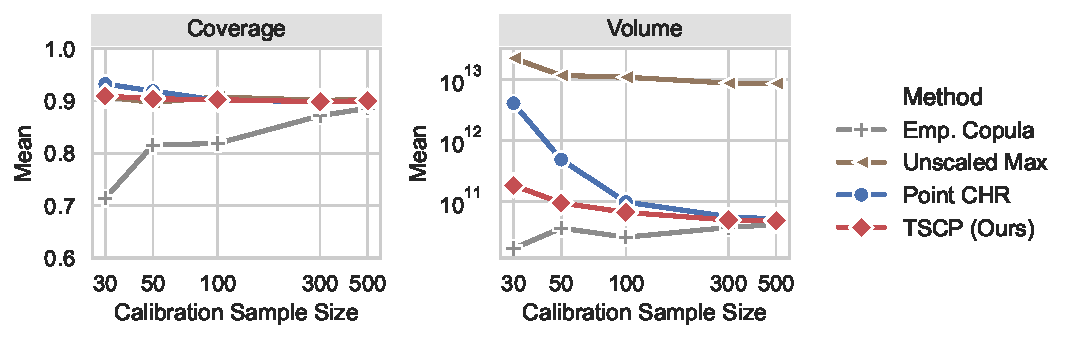
\includegraphics[width=0.9\textwidth]{figures/baselines/gaussian_10d.pdf} 
\caption{Average performance of the proposed TSCP method and alternative conformal prediction approaches on simulated data with $d=10$ outcome variables and heterogeneous noise variances. The target coverage level is $90\%$. TSCP consistently attains near-nominal coverage while producing the smallest prediction sets on average. Numerical results and corresponding standard deviations are reported in Table~\ref{tab:gaussian-heter}. }
     \label{fig:gaussian-heter}
\end{figure}


These results show that our method performs well across both small and large sample sizes, with empirical coverage close to $1-\alpha$, using relatively tight prediction sets.
The \emph{Point CHR} approach yields substantially larger, and therefore less informative, prediction sets—especially in small samples (e.g., $n < 100$)—due to the inefficiency introduced by its additional sample split. Even for moderately large samples, our method continues to perform noticeably better, although this difference is difficult to discern in Figure~\ref{fig:gaussian-heter} because of the log–log scale; see Table~\ref{tab:gaussian-heter} for a more detailed numerical summary.
The \emph{Emp.~Copula} approach clearly fails to achieve finite-sample coverage, since it uses the same calibration set both to estimate the copula model and to calibrate the prediction sets based on the resulting nonconformity scores. While this issue could be addressed through additional data splitting, doing so would come with the same efficiency disadvantages of \emph{Point CHR}. This limitation is shared by related copula-based approaches that we do not explicitly include in our comparisons.
Finally, the \emph{Unscaled Max} approach produces much larger (and effectively uninformative) prediction sets in both small and large samples, as it is negatively affected by the unequal variances of the noise distribution across different dimensions.


Figure~\ref{fig:gaussian-homo} reports results from analogous experiments in which the noise distribution has equal variance across dimensions, with $\epsilon^{\mathrm{homo}}_j \sim \mathcal{N}(0, 1)$ for all $j \in [10]$. This setting strongly favors the \emph{Unscaled Max} approach; nevertheless, our TSCP still performs as a close second.
In practice, however, noise levels are rarely known \emph{a priori}, making the adaptivity and robustness of TSCP generally desirable.


\begin{figure}[!htbp]
    \centering
    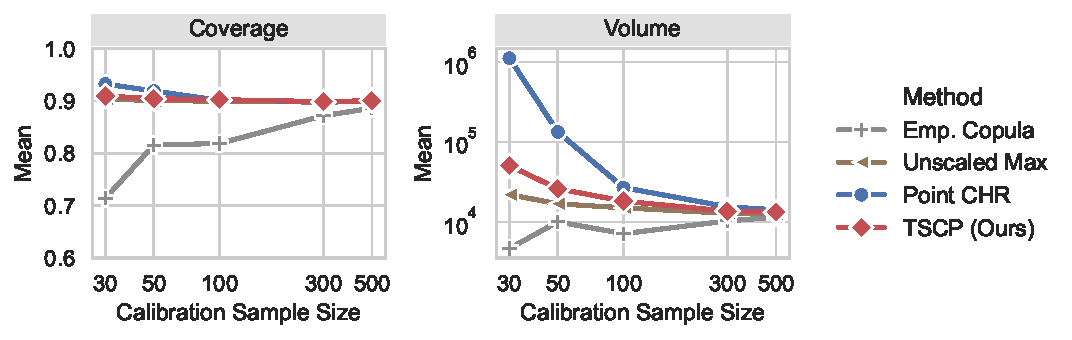
\includegraphics[width=0.9\textwidth]{figures/baselines/unit_gaussian_10d.pdf}
\caption{Average performance of the proposed TSCP method and alternative conformal prediction approaches in numerical experiments similar to those of Figure~\ref{fig:gaussian-heter}. Here, the outcome variables have homogeneous variance across their $d=10$ dimensions, which gives an advantage to the \emph{Unscaled Max} approach. The target coverage level is $0.9$. TSCP attains near-nominal coverage and is competitive, while Unscaled Max is the most efficient in this homogeneous setting. Numerical results and corresponding standard deviations are reported in Table~\ref{tab:gaussian-homo}.}
     \label{fig:gaussian-homo}
\end{figure}

The results of additional numerical experiments are reported in Appendices~\ref{app:ours_simulation}--\ref{app:hevy_tailed_simulation}. In Appendix~\ref{app:ours_simulation}, we compare TSCP with several alternative approaches described in Sections~\ref{sec:preliminaries} and~\ref{sec:methods}, including the naive plug-in rescaling procedure (Algorithm~\ref{alg:std-plug-in}), the data-splitting variant (Algorithm~\ref{alg:std-ds}), the conservative global worst-case approach (Algorithm~\ref{alg:global}), and the union-based construction without rectangular enclosure (Section~\ref{sec:method-lwc}). These experiments highlight the favorable balance between statistical–computational trade-offs achieved by TSCP. We further examine scalability with respect to the outcome dimension and show that Algorithm~\ref{alg:shortcut} remains computationally efficient in regimes where union-based constructions become prohibitive. In Appendix~\ref{app:hevy_tailed_simulation}, we investigate the robustness of TSCP under heavy-tailed noise and demonstrate that our method has near-nominal empirical coverage in the displayed infinite-variance cases; this is a stress test outside Assumption~\ref{eq:assumption-scores}, not a theoretical extension.

\subsection{Experiments with Real Data}

We now evaluate all methods on six real datasets. 
The first four, \emph{rf2} \citep{grigorios_tsoumakas_eleftherios_spyromitros-xioufis_william_groves_ioannis_vlahavas_2022}, \emph{scm1d} \citep{scm1d}, \emph{scm20d} \citep{scm20d}, and \emph{stock} \citep{stock_portfolio_performance_390}, are borrowed from related prior works \citep{pmlr-v258-park25c, dheur2025unified}. 
The other two datasets, \emph{student} \citep{cortez2008student} and \emph{energy} \citep{tsanas2012energy}, are obtained from the UCI repository and serve to illustrate the small-sample performance of TSCP.

For each dataset, we perform $200$ random train/calibration/test splits using a $75\%/5\%/20\%$ ratio. We fit a multivariate sparse (lasso) regression model with regularization parameter $\lambda = 0.0001$ on \emph{stock}, and random forest regression models on all other datasets; see the GitHub software repository linked in the Software Availability section for additional reproducibility details.
Table~\ref{tab:real} reports the average coverage and volume, along with one standard deviation.
As shown in Table~\ref{tab:real}, the empirical behavior of all methods on real data largely mirrors the trends observed in the simulation studies. Among methods with theoretical coverage guarantees, TSCP achieves the smallest prediction-set volume on the \emph{stock}, \emph{scm1d}, \emph{scm20d}, and \emph{energy} datasets. On \emph{rf2}, TSCP is outperformed by \emph{Point CHR}, likely due to the presence of a small number of influential outliers. On \emph{student}, \emph{Unscaled Max} yields smaller volumes, consistent with the approximately homogeneous noise across targets (student GPAs at different grade levels).
The \emph{Point CHR} approach produces an uninformative, \emph{infinite} prediction set on the \emph{stock} dataset, because its additional data split makes the effective calibration set extremely small.
Finally, \emph{Emp.~Copula} generally fails to achieve the desired coverage level, consistent with its lack of finite-sample guarantees.
Overall, the results show that TSCP provides a reasonable trade-off between coverage and volume, excelling especially when calibration data are limited or when noise scales differ significantly across targets.

\begin{table}[!htbp]
\centering
\captionsetup[subtable]{justification=centering}
\small
\begin{subtable}{\textwidth}
\centering
\begin{tabular}[t]{l c c c c }
\toprule
\textbf{Method} & \multicolumn{2}{c}{Stock $(d=6,\, n=15)$} & \multicolumn{2}{c}{rf2 $(d=8,\, n=384)$} \\
\cmidrule(lr){2-3}\cmidrule(lr){4-5}
& Coverage & Volume & Coverage & Volume \\
\midrule
Unscaled Max & 0.940(0.057) & 6.03e-02(1.57e-01) & 0.900(0.016) & 4.14e+03(2.90e+03) \\
Emp. copula & \color{red}0.727(0.113) & 1.01e-05(9.80e-06) & \color{red}{0.893(0.016)} & 5.35e+01(4.69e+01) \\
Point CHR & 1.000(0.000) & \text{inf} & 0.901(0.022) & \textbf{{6.85e+01(7.55e+01)}} \\
TSCP & 0.956(0.059) & \textbf{{1.86e-03(8.55e-03)}} & 0.901(0.017) & 5.42e+02(1.50e+03) \\
\midrule

\end{tabular}
%\subcaption{First panel: Stock, rf2.}
\end{subtable}

\small
\begin{subtable}{\textwidth}
\centering
\begin{tabular}[t]{l c c c c }
\midrule
\textbf{Method} & \multicolumn{2}{c}{scm1d $(d=16,\, n=490)$} & \multicolumn{2}{c}{scm20d $(d=16,\, n=448)$} \\
\cmidrule(lr){2-3}\cmidrule(lr){4-5}
& Coverage & Volume & Coverage & Volume \\
\midrule
Unscaled Max & 0.900(0.016) & 2.74e+39(4.02e+39) & 0.901(0.016) & 2.70e+40(2.92e+40) \\
Emp. copula & \color{red}{0.893(0.016)} & 1.09e+39(1.34e+39) & \color{red}{0.892(0.017)} & 1.178e+40(1.190e+40) \\
Point CHR & 0.905(0.020) & 2.84e+39(5.43e+39) & 0.902(0.023) & 3.00e+40(8.00e+40) \\
TSCP & 0.901(0.015) & \textbf{{1.52e+39(2.61e+39)}} & 0.901(0.016) & \textbf{{1.53e+40(1.50e+40)}} \\
\midrule

\end{tabular}
%\subcaption{Second panel: scm1d, scm20d.}
\end{subtable}

\small
\begin{subtable}{\textwidth}
\centering
\begin{tabular}[t]{l c c c c }
\midrule

\textbf{Method} & \multicolumn{2}{c}{Energy $(d=2,\, n=38)$} & \multicolumn{2}{c}{Student $(d=3,\, n=32)$} \\
\cmidrule(lr){2-3}\cmidrule(lr){4-5}
& Coverage & Volume & Coverage & Volume \\
\midrule
Unscaled Max & 0.917(0.049) & 1.58e+01(6.80e+00) & 0.904(0.055) & \textbf{{1.51e+02(1.27e+02)}} \\
Emp. copula & \color{red}0.886(0.061) & 5.41e+00(4.49e+00) & \color{red}0.861(0.073) & 1.08e+02(7.19e+01) \\
Point CHR & 0.899(0.069) & 8.81e+00(2.42e+01) & 0.939(0.057) & 6.89e+02(1.07e+03) \\
TSCP & 0.922(0.048) & \textbf{{6.95e+00(4.43e+00)}} & 0.912(0.056) & 1.98e+02(1.77e+02) \\

\bottomrule
\end{tabular}
%\subcaption{Third panel: Energy, Student.}
\end{subtable}

\caption{Performance of the proposed TSCP method and alternative conformal prediction approaches on real datasets. Results are averaged over $200$ random splits of the data into training/calibration/and test subsets, with one standard deviation reported in parentheses. The target coverage level is $0.9$. Coverage values below the target are highlighted in \textcolor{red}{red}, and the smallest volume among methods achieving valid coverage is highlighted in \textbf{bold}.}
\label{tab:real}
\end{table}

\FloatBarrier
\subsection{Retained Distribution-Specific Results}
\label{app:legacy-supplement}

This section presents the results of additional numerical experiments, including comparisons with a broader range of alternative approaches.
These experiments are conducted using the same protocol and performance metrics described in Appendix~\ref{app:legacy-experiments} unless specified otherwise. 

\subsubsection{Distribution-Specific Tables}
\label{app:simulations}

Here we present additional results from the numerical experiments described in Appendix~\ref{app:legacy-experiments}, corresponding to five noise settings. These results are qualitatively consistent with those summarized in Appendix~\ref{app:legacy-experiments}: our method performs consistently well, producing relatively tight prediction sets with near-nominal empirical coverage.

\subsubsection*{Gaussian Noise (heterogeneous)}

\begin{table}[H]
    \centering
    \input{figures/baselines/gaussian_10d_table}
    \caption{Performance of the proposed TSCP method and alternative conformal prediction approaches on simulated data with $d=10$ outcome variables, as in Figure~\ref{fig:gaussian-heter}. All results are averaged over $200$ trials with their one standard deviation reported in parenthesis.  
    The target coverage level is $0.9$. Coverage below this target is highlighted in \textcolor{red}{red}. For volume, lower is better. Smallest volume size (among those with valid theoretical coverage) is highlighted in \textbf{bold}. TSCP yields the tightest volume while maintaining valid coverage.}
    \label{tab:gaussian-heter}
\end{table}

\clearpage
\subsubsection*{Gaussian Noise (homogeneous)}

\begin{table}[H]
    \centering
    \input{figures/baselines/unit_gaussian_10d_table}
    \caption{Performance of the proposed TSCP method and alternative conformal prediction approaches on simulated data with $d=10$ outcome variables, as in Figure~\ref{fig:gaussian-homo}. Other details are as in Table~\ref{tab:gaussian-heter}. In this case, Unscaled Max yields the tightest volume while maintaining valid coverage, while TSCP remains a competitive second. }
    \label{tab:gaussian-homo}
\end{table}

\clearpage
\subsubsection*{Laplace Noise}
\begin{table}[H]
    \centering
    \input{figures/baselines/laplace_10d_table}
    \caption{Performance of the proposed TSCP method and alternative conformal prediction approaches on simulated data with $d=10$ outcome variables, and noise following a \emph{Laplace} distribution; i.e., $\epsilon _j \sim \mathrm{Laplace}(10-j+1)$ for all $j \in [10]$. Other details are as in Table~\ref{tab:gaussian-heter}.}
    \label{tab:laplace}
\end{table}

\clearpage
\subsubsection*{Mixture Noise}

\begin{table}[H]
    \centering
    \input{figures/baselines/mixed_10d_table}
    \caption{Performance of the proposed TSCP method and alternative conformal prediction approaches on simulated data with $d=10$ outcome variables, and noise following a \emph{Mixture} distribution; i.e., $\epsilon_j \sim \frac{1}{2}\mathrm{Laplace}(10-j+1)+\frac{1}{2}\mathcal{N}(0, (10-j+1)^2)$ for all $j \in [10]$. Other details are as in Table~\ref{tab:gaussian-heter}.}
    \label{tab:mixed}
\end{table}

\clearpage
\subsubsection*{Gamma Noise}
 
\begin{table}[H]
    \centering
    \input{figures/baselines/gamma_10d_table}
    \caption{Performance of the proposed TSCP method and alternative conformal prediction approaches on simulated data with $d=10$ outcome variables, and noise following a \emph{Gamma} distribution; i.e., $\epsilon_j \sim  \mathrm{Gamma}(1, 10-j+1)$ for all $j \in [10]$. Other details are as in Table~\ref{tab:gaussian-heter}.}
    \label{tab:gamma}
  \end{table}

\clearpage
  \subsection{Comparison of Alternative Implementations of TSCP}
\label{app:ours_simulation}

The additional methods considered in this section include (i) \emph{Naive}, the heuristic plug-in rescaling method that uses location and scale parameters estimated directly from the calibration data without further adjustments, summarized in Algorithm~\ref{alg:std-plug-in}; (ii) \emph{TSCP-S}, the inefficient data-splitting variant summarized in Algorithm~\ref{alg:std-ds}; (iii) \emph{TSCP-GWC}, our conservative global-worst-case method summarized in Algorithm~\ref{alg:global}; (iv) \emph{TSCP-LWC}, the aggregated union described in Section~\ref{sec:method-lwc} but not enclosed by a rectangle. 


\begin{figure}[!htbp]
    \begin{subfigure}[b]{\textwidth}
        \centering
        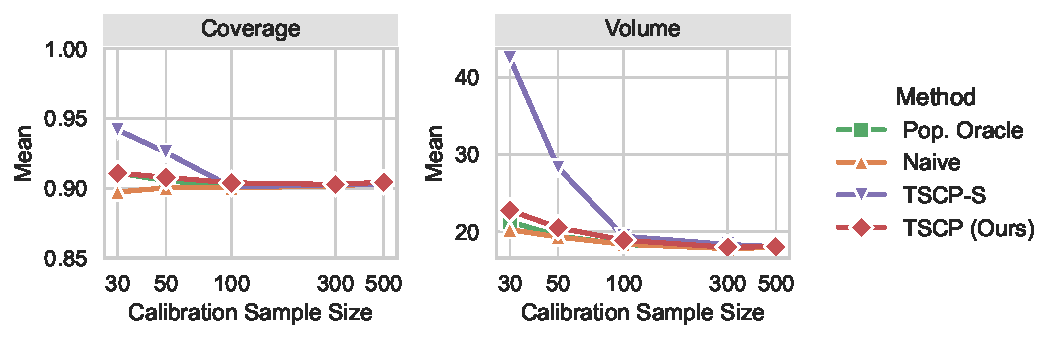
\includegraphics[width=0.9\textwidth]{figures/ours/ours_approximation_2d.pdf}
    \end{subfigure}
    \begin{subfigure}[b]{\textwidth}
        \centering
        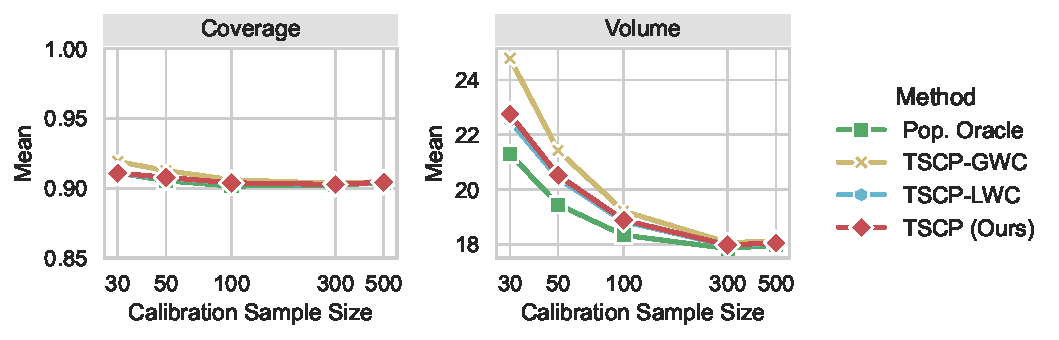
\includegraphics[width=0.9\textwidth]{figures/ours/ours_containment_2d.pdf}
    \end{subfigure}
    \caption{Performance of TSCP and alternative approaches on simulated data with $d=2$ targets and heterogeneous Laplace noise. The target coverage level is $90\%$. Results are averaged over $200$ trials. All methods achieve near-nominal coverage and approximate \emph{Pop.~Oracle} as the calibration sample size increases. TSCP tracks TSCP-LWC closely, with an almost indistinguishable average volume, highlighting the tightness of its rectangular enclosure.}
    \label{fig:approximation1}
\end{figure}

All methods compared in Figure~\ref{fig:approximation1} tend to approximate \emph{Pop.~Oracle} well as $n$ increases, with TSCP and TSCP-LWC being the two most stable and fastest approximations among all methods with theoretical coverage. These results also show that TSCP encloses the aggregated union TSCP-LWC very tightly, and that TSCP-GWC is conservative, though it still performs better than the data-splitting variant TSCP-S. Despite lacking a finite-sample coverage guarantee, the \emph{Naive} approach performs well, as also shown in Figure~\ref{fig:approximation2}.

\begin{figure}[!htbp]
    \centering
    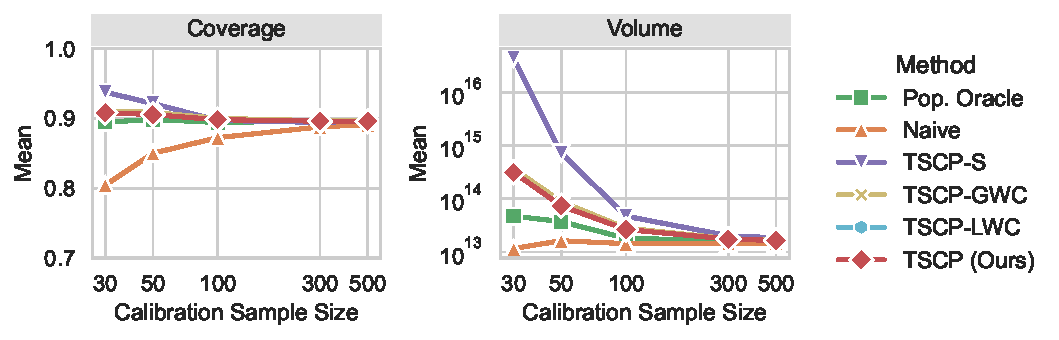
\includegraphics[width=0.9\textwidth]{figures/ours/ours_containment_10d.pdf}
    \caption{Performance of TSCP and alternative approaches on simulated data with $d=10$ targets. Other details are as in Figure~\ref{fig:approximation1}. TSCP-LWC is omitted from this figure due to its prohibitive cost with even moderately high-dimensional outcomes.}
    \label{fig:approximation2}
\end{figure}

Figure~\ref{fig:runtime} better highlights the prohibitive computational cost of TSCP-LWC, by reporting on the results of similar experiments where a small sample size is fixed, $|\mathcal{D}_{\mathrm{cal}}|=30$, while the outcome dimensions are gradually increased: $d \in \{2, 3, 4, 5, 10, 20, 30\}$.

\begin{figure}[!htbp]
    \centering
    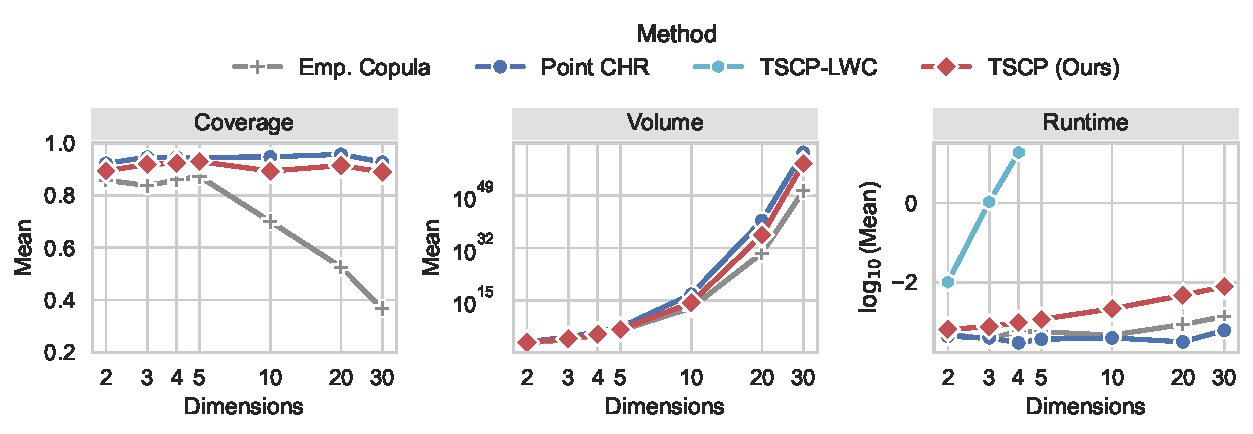
\includegraphics[width=\textwidth]{figures/ours/ours_runtime.pdf}
    \caption{Performance of TSCP and alternative approaches on simulated data with fixed sample size $|\mathcal{D}_{\mathrm{cal}}|=30$, as a function of the number of output dimensions $d$. Other details are as in Figure~\ref{fig:approximation1}. These results are averaged over $30$ repetitions under the original resampling protocol. The runtime results are presented in seconds on a $\log_{10}$ scale. 
    The runtime of all methods except TSCP-LWC scales well with number of dimensions. TSCP-LWC is only applied when $d \in \{2,3,4\}$ due to the exponential growth of its runtime. }
    \label{fig:runtime}
\end{figure}

\clearpage
\subsection{Robustness to Heavy-Tailed Data} \label{app:hevy_tailed_simulation}


We test the performance of TSCP on simulated heavy-tailed data with $d=10$ outcomes and noise following a Student's-$t$ distribution; i.e., $Y_j \mid \mathbf X \sim f_j(\mathbf X) + \epsilon_j$ with $\epsilon_j \sim t_{\mathrm{DF}}$ and $\mathrm{DF} \in \{1.5,2,3\}$ degrees of freedom. 
For $1 < \mathrm{DF} \leq 2$, the Student's-$t$ distribution leads to residuals with infinite population variance, violating Assumption~\ref{eq:assumption-scores}. The plotted empirical coverage remains near the target in these cases. This observation does not extend the validity theorem beyond its assumptions, and the large volumes show a substantial loss of informativeness.


\begin{figure}[!htbp]
     \centering
     \begin{subfigure}[b]{\textwidth}
         \centering
         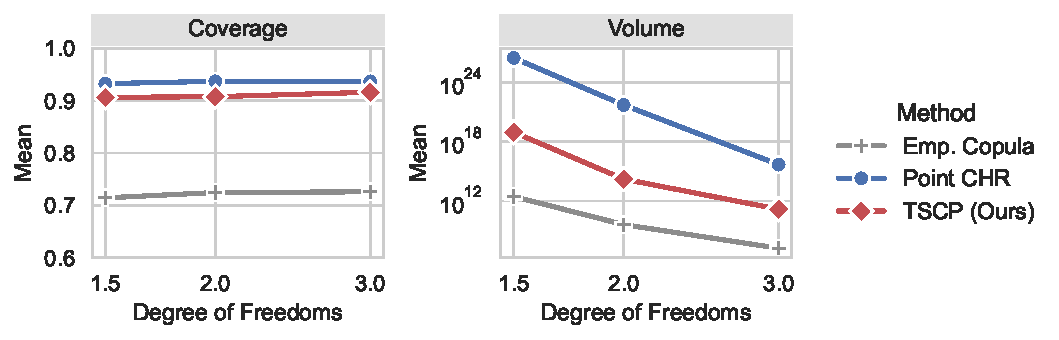
\includegraphics[width=0.9\textwidth]{figures/t/t_n30_10d.pdf}
         \caption{Small sample, $|\mathcal{D}_{\mathrm{cal}}|=30$. Output dimensions $d=10$.}
         \label{fig:t-n30-10d}
     \end{subfigure}
     \vfill
     \begin{subfigure}[b]{\textwidth}
         \centering
         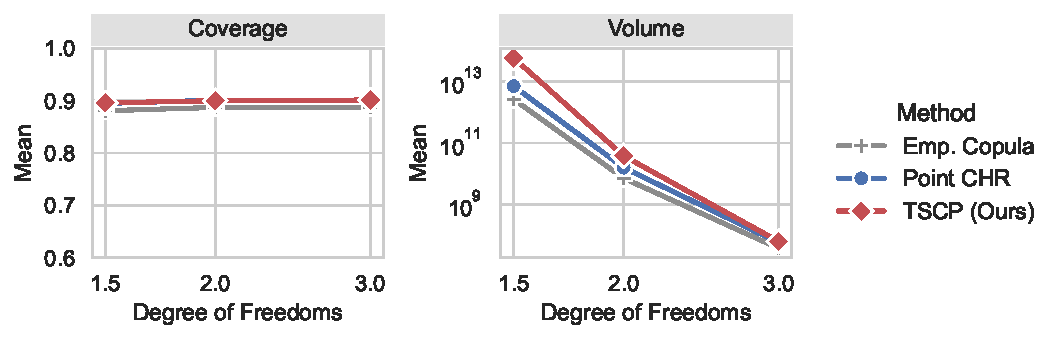
\includegraphics[width=0.9\textwidth]{figures/t/t_n500_10d.pdf}
         \caption{Large sample, $|\mathcal{D}_{\mathrm{cal}}|=500$. Output dimensions $d=10$.}
         \label{fig:t-n500-10d}
     \end{subfigure}
        \caption{Performance of the proposed TSCP method and other approaches on simulated data with noise following a Student's-$t$ distribution with varying degrees of freedom, using small (a) and large (b) sample sizes. The target coverage level is 0.9. All methods except \emph{Emp.~Copula} have near-nominal coverage in all settings. TSCP has near-nominal empirical coverage in these displayed heavy-tail cases; the infinite-variance cases are outside the stated assumptions. In the small sample setting, Point CHR suffers more in terms of prediction set size due to its inefficient use of calibration data, although it can outperform TSCP in large samples.}
        \label{fig:t}
\end{figure}
 
% \begin{table}
%     \centering
%     \input{figures/t/t_n30_10d}
%     \caption{Performance on Student's-$t$ distribution with varying degree of freedoms on small sample size $|\mathcal{D}_{\mathrm{cal}}|=30$. This table contains all data used to generate Figure~\ref{fig:t-n30-10d} along with one standard deviation of the test coverage and volume over $200$ trials. Target coverage is $0.9$. Coverage below this target is highlighted in \textcolor{red}{red}. For volume, lower is better. Smallest volume size (among those with valid coverage) is highlighted in \textcolor{red}{red}. }
%     \label{tab:t-n30-10d}
% \end{table}

% \begin{table}
%     \centering
%     \input{figures/t/t_n500_10d}
%     \caption{Performance on Student's-$t$ distribution with varying degree of freedoms on large sample size $|\dataset_{\mathrm{cal}}|=500$. This table contains all data used to generate Figure~\ref{fig:t-n500-10d} along with one standard deviation of the test coverage and volume over $200$ trials. Target coverage is $0.9$. Coverage below this target is highlighted in \textcolor{red}{red}. For volume, lower is better. Smallest volume size (among those with valid coverage) is highlighted in \textcolor{red}{red}. Point CHR has the smallest volume while maintaing valid coverage when the degree of freedom is less than $3$, but when systematic outliers getting removed as the degree of freedom increases, our TSCP becomes the one with the smallest volume while maintaining valid coverage. }
%     \label{tab:t-n500-10d}
% \end{table}



%%% Local Variables:
%%% mode: latex
%%% TeX-master: "main"
%%% End:
\FloatBarrier
\endgroup
